\documentclass[a4paper,12pt]{report}

% Page layout
\usepackage[left=2.5cm,right=2.5cm,top=2.5cm,bottom=2.5cm]{geometry}

% Figures
\usepackage[margin=\the\parindent,small,bf,sf]{caption}
\usepackage{graphicx}
\usepackage{pdfpages}
\setlength{\abovecaptionskip}{7.5pt}  % spacing above and below captions
\newcommand*{\WaterMark}[2][0.2\paperwidth]{\AddToShipoutPicture*{\AtTextCenter{\parbox[c]{0pt}{\makebox[0pt][c]{\includegraphics[width=#1]{#2}}}}}}

% Font and text
\usepackage[english]{babel}
\usepackage{microtype}
\usepackage{setspace}
\usepackage{lmodern}
\newcommand{\myemph}[1]{{\sffamily\bfseries#1}}
\sloppy
\onehalfspacing

% Headings
\usepackage[raggedright,sf,bf]{titlesec}
\titlelabel{\thetitle.\ }
\titleformat{\chapter}[display]{\huge\bfseries\sffamily}{\chaptertitlename\ \thechapter}{15pt}{\Huge \raggedright}
% \titleformat{\chapter}[display]{\centering\huge\bfseries\sffamily}{\chaptertitlename\ \thechapter:}{15pt}{}
\titlespacing*{\chapter}{0pt}{0pt}{40pt}  % remove spacing before chapter headings

% Table of contents
\makeatletter
\let\originall@chapter\l@chapter
\def\l@chapter#1#2{\originall@chapter{{\sffamily #1}}{#2}}
\makeatother
\let \savenumberline \numberline
\def \numberline#1{\savenumberline{#1.}}

% Mathematics
\usepackage[cmex10]{amsmath}
\usepackage{amssymb}
\usepackage{cancel}
\DeclareMathOperator*{\argmax}{arg\,max}
\newcommand{\T}{^\textrm{T}}
\newcommand{\tr}{\textrm{tr}}
\renewcommand{\vec}[1]{\boldsymbol{\mathbf{#1}}}
\newcommand{\defeq}{\triangleq}

% Tables
\usepackage{booktabs}
\usepackage{tabularx}
\usepackage{multirow}
\newcommand{\mytable}{
    \centering
    \small
    \renewcommand{\arraystretch}{1.2}
    }
\renewcommand{\tabularxcolumn}[1]{m{#1}}
\newcolumntype{C}{>{\centering\arraybackslash}X}
\newcolumntype{L}{>{\raggedright\arraybackslash}X}

% Header and footer
\usepackage{fancyhdr}
\pagestyle{fancy}
\fancyhf{}
\renewcommand{\sectionmark}[1]{\markright{\normalsize \thesection.\ #1}}
\fancyhead[C]{\nouppercase{\textit{\rightmark}}}
\fancyhead[RO]{\thepage}
% \fancyhead[LE]{\thepage}  % double-sided printing
\fancyfoot{}
\setlength\headheight{14.5pt}
\renewcommand{\headrulewidth}{0pt}
\fancypagestyle{plain}{\fancyhead{}
                       \renewcommand{\headrulewidth}{0pt}
                       \fancyfoot[C]{\thepage}}

% Pseudo-code
\usepackage{algorithm}  % should go before \usepackage{hyperref}

% Table of contents and hyperlinks
\usepackage{hyperref}
\hypersetup{colorlinks=true,linktoc=all,citecolor=black,linkcolor=black}
\usepackage[nottoc]{tocbibind}

% Pseudo-code
\usepackage{algpseudocode}  % should go after \usepackage{hyperref}
\renewcommand{\thealgorithm}{\arabic{chapter}.\arabic{algorithm}} 
%\captionsetup[algorithm]{labelfont={bf,sf},font=small,labelsep=colon}

% Bibliography
\usepackage{cite}  % automatically reorder inline citations
\bibliographystyle{IEEEtran}

% Fix titlesec issue
\usepackage{etoolbox}
\makeatletter
\patchcmd{\ttlh@hang}{\parindent\z@}{\parindent\z@\leavevmode}{}{}
\patchcmd{\ttlh@hang}{\noindent}{}{}{}
\makeatother


\begin{document}

% Front matter
\graphicspath{{frontmatter/fig/}}
\pagenumbering{Alph}

\begin{titlepage}
\begin{center}


\includegraphics[width=10cm]{USlogo-top}

\vfill

{\sffamily \bfseries \huge A critical analysis of major design flaws in the Death Star \par}

\vfill

{\large {\Large Obi-Wan Kenobi} \\ 99652154 \par}

\vfill

\vfill

{Report submitted in partial fulfilment of the requirements of the module \\
Project (E) 448 for the degree Baccalaureus in Engineering in the Department of
Electrical and Electronic Engineering at Stellenbosch University. \par}

\vfill

{\large {Supervisor}: Dr L. Skywalker} %\\
% Department of Electrical and Electronic Engineering \par}

\vfill

{\Large October 2099}
\end{center}
\end{titlepage}

%\graphicspath{{frontmatter/fig/}}
\pagenumbering{Alph}

\begin{titlepage}
\begin{center}

%
\includegraphics[width=10cm]{USlogo-top}

\WaterMark{UScrest-WM}

~\vspace{4.5em}

{\sffamily \bfseries \huge A critical analysis of major design flaws in the Death Star \par}

\vspace{7em}

{\large {\Large Obi-Wan Kenobi} \\ 99652154 \par}

\vspace{8em}

{\large Thesis presented in partial fulfilment of the requirements for the degree of \\ Master of Engineering (Electronic) in the Faculty of Engineering at Stellenbosch University. \par}

\vfill

{\large {Supervisor}: Dr H. Kamper \\
Department of Electrical and Electronic Engineering \par}

%\vfill
\vspace{10em}

{\Large October 2099}
\end{center}
\end{titlepage}

\pagenumbering{roman}
\chapter*{Acknowledgements}
% \addcontentsline{toc}{chapter}{Acknowledgements}
\makeatletter\@mkboth{}{Acknowledgements}\makeatother

I would like to thank my dog, Muffin. I also would like to thank the inventor of the incubator; without him/her, I would not be here. Finally, I would like to thank Dr Herman Kamper for this amazing report template.
%\chapter*{Declaration}
\newpage
\pagestyle{plain}
\addcontentsline{toc}{chapter}{Declaration}
\makeatletter\@mkboth{}{Declaration}\makeatother

\centerline{
\includegraphics[width=8cm]{USlogo-top}}
\vspace*{-10pt}

\section*{\centering Plagiaatverklaring / \textit{Plagiarism Declaration}}

\vspace*{5pt}

\begin{enumerate}
    \item Plagiaat is die oorneem en gebruik van die idees, materiaal en ander intellektuele eiendom van ander persone asof dit jou eie werk is.\\
    \textit{Plagiarism is the use of ideas, material and other intellectual property of another's work
        and to present is as my own.}
    
    \item Ek erken dat die pleeg van plagiaat 'n strafbare oortreding is aangesien dit 'n vorm van diefstal is.\\
    \textit{I agree that plagiarism is a punishable offence because it constitutes theft.}
    
    \item Ek verstaan ook dat direkte vertalings plagiaat is. \\
    \textit{I also understand that direct translations are plagiarism.}
    
    \item Dienooreenkomstig is alle aanhalings en bydraes vanuit enige bron (ingesluit die internet) volledig verwys (erken). Ek erken dat die woordelikse aanhaal van teks sonder aanhalingstekens (selfs al word die bron volledig erken) plagiaat is. \\
    \textit{Accordingly all quotations and contributions from any source whatsoever (including the internet) have been cited fully. I understand that the reproduction of text without quotation marks (even when the source is cited) is plagiarism}
    
    \item Ek verklaar dat die werk in hierdie skryfstuk vervat, behalwe waar anders aangedui, my eie oorspronklike werk is en dat ek dit nie vantevore in die geheel of gedeeltelik ingehandig het vir bepunting in hierdie module/werkstuk of 'n ander module/werkstuk~nie. \\
    \textit{I declare that the work contained in this assignment, except where otherwise stated, is my original work and that I have not previously (in its entirety or in part) submitted it for grading in this module/assignment or another module/assignment.}
\end{enumerate}

\vfill

\noindent \begin{tabularx}{1.0\linewidth}{|L|L|}
    \hline
    \vspace{1cm} {Studentenommer / \textit{Student number}} & \vspace{1cm} {Handtekening / \textit{Signature}} \\
    \hline
    \vspace{1cm} {Voorletters en van / \textit{Initials and surname}} & \vspace{1cm} {Datum / \textit{Date}} \\
    \hline
\end{tabularx}

\vspace{15pt}

% The old declaration

%I, the undersigned, hereby declare that the work contained in this report is my own original work unless otherwise stated.
%
%% Afrikaans:
%% Hiermee verklaar ek, die ondergetekende, dat die werk in hierdie verslag vervat my eie oorspronklike werk is, tensy anders vermeld.
%
%\vspace{2.5cm}
%
%\begin{table}[h]
%\begin{tabular}{@{}p{2.5cm}p{5cm}}
%    Signature: & \dotfill \\
%    & \multicolumn{1}{c}{Obi-Wan Kenobi} \\
%    ~\vspace{1cm} \\
%    Date: & \dotfill \\
%\end{tabular}
%\end{table}
%
%\vfill
%
%\begin{center}
%    Copyright \textcopyright\ 2099 Stellenbosch University \\
%    All rights reserved
%\end{center}


\chapter*{Abstract}
\addcontentsline{toc}{chapter}{Abstract}
\makeatletter\@mkboth{}{Abstract}\makeatother

\subsubsection*{English}

The English abstract.

\selectlanguage{english}
\tableofcontents
\listoffigures
\listoftables
\chapter*{Nomenclature\markboth{}{Nomenclature}}
\addcontentsline{toc}{chapter}{Nomenclature}

% \vspace*{-3mm}
\subsubsection*{Variables and functions}

\begingroup
\renewcommand{\arraystretch}{1.2}
\renewcommand{\tabularxcolumn}[1]{p{#1}}
\begin{tabularx}{\textwidth}{@{}p{2.5cm}L}
    $p(x)$ & Probability density function with respect to variable $x$.\\
\end{tabularx}
\endgroup

\subsubsection*{Acronyms and abbreviations}

\begingroup
\renewcommand{\arraystretch}{1.2}
\begin{tabular}{@{}p{2.5cm} l}
    RL		& Reinforcement Learning \\
    SARSA	& State-Action-Reward-State=Action \\
    Q-learning	& Q value learning \\
    MDP		& Markov Decision
    Process \\
\end{tabular}
\endgroup

\newpage
\pagenumbering{arabic}

% Contents
\graphicspath{{introduction/fig/}}

\chapter{Introduction}
\label{chap:introduction}

\section{Problem Statement and Project Objective}
In robotics, a manipulator (ie. a robotic arm) is a device used to manipulate objects in its environment. When the manipulation task is relatively complex, it is often difficult or even impossible for a human to direct how the robot should act. One possible solution is that the robot learn by itself which actions are best, which can be done through reinforcement learning. A popular method for doing developing reinforcement learning algorithms for robotics is to first solve similar, less complex problems.

In this project reinforcement learning is used to solve sliding puzzle. An example of a sliding puzzle being solved can be seen in Figure \ref{fig:sliding_puzzle_figs}. The objective of this project is to solve a shuffled puzzle with the minimum amount of moves using reinforcement learning. The rules of the game are explained in the next section. 

\section{Background}

The sliding puzzle is a game with a history dating back to the 1870's \cite{15_puz}. The game consists of $N^{2}-1$ tiles arranged on an NxN grid with one empty tile. The tiles are numbered 1 to N. A possible configuration of a 3x3 puzzle is shown in Figure \ref{fig:sfig1}. The puzzles state can be changed by sliding one of the numbered tiles, next to the empty tile, into the place of the empty tile. The empty tile then takes the place of the numbered tile. This can visually be seen between Figures \ref{fig:sfig1}
and \ref{fig:sfig2} where tile number 6 moves right in the transition between Figures \ref{fig:sfig1}
and \ref{fig:sfig2}. We will denote the action that can occur in a certain state by the possible movements the empty tile can move. Which will be defined as $A_s = {up, down, left, right}$.

The sliding puzzle is a game with a history dating back to the 1870's \cite{15_puz}. Many solutions have been thought up to solve such puzzles, which include using search algorithms\cite{search_alg}. The rules of the game are that the only tiles that can move are the ones next to the tile with no number, known as the 'blank tile'. Additionally only one tile can be moved at a time. The final puzzle configuration is shown in \ref{fig:sfig4}, where all the tiles are placed in ascending order read left to right and top to bottom. The aim of the game is to arrange a shuffled puzzle into the final puzzle configuration by moving one tile at a time.

\begin{figure}[!htb]
	\centering
	\begin{subfigure}{.4\textwidth}
		\centering
		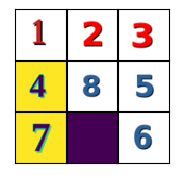
\includegraphics[width=.8\linewidth]{game_states/31.png}
		\caption{Puzzle with tiles 5,6,8 and blank in the incorrect positions}
		\label{fig:sfig1}
	\end{subfigure}%
	\begin{subfigure}{.4\textwidth}
		\centering
		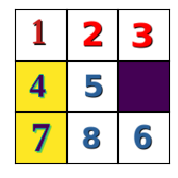
\includegraphics[width=.8\linewidth]{game_states/32.png}
		\caption{Puzzle with tiles 5,8 and blank in the incorrect positions}
		\label{fig:sfig2}
	\end{subfigure}
	\begin{subfigure}{.4\textwidth}
		\centering
		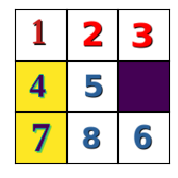
\includegraphics[width=.8\linewidth]{game_states/33.png}
		\caption{Puzzle with tiles 8 and blank in the incorrect positions}
		\label{fig:sfig3}
	\end{subfigure}
	\begin{subfigure}{.4\textwidth}
		\centering
		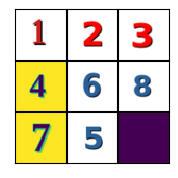
\includegraphics[width=.8\linewidth]{game_states/34.png}
		\caption{Solved puzzle}
		\label{fig:sfig4}
	\end{subfigure}
	\caption{Figures of a 3x3 sliding puzzle being solved}
	\label{fig:sliding_puzzle_figs}
\end{figure}

\section{Document Outline} 
In Chapter \ref{chap:Literature_Review} we will look at a paper which used an alternate approach to solve a 16 tile sliding puzzle.
Chapter \ref{chap:MDP} describes in detail theory relating to Markov decision processes.
Chapter \ref{chap:RL} discusses in detail the dynamic programming and reinforcement learning techniques which will be used to solve our puzzle problem.

In Chapter \ref{chap:System_Design} the theory of reinforcement learning is applied to solve sliding puzzles. In the same chapter we 

{\color{red}Rather how you used the theory of RL to design the solution to the sliding puzzle problem. Do this mathematically. Talk about things like the size of the state space, the sequential agents that you trained, how you decided on algorithms or hyperparameters.}

Chapter \ref{chap:Experiments_and_Results} contains tests and verification that our solution works using the results of various experiments.
Chapter \ref{chap:conclusion} concludes the report.
\graphicspath{{chapter2/fig}}
\chapter{Solvability of a NxN sliding puzzle}
\label{chap:Solvability of a NxN sliding puzzle}
\section{General puzzle description}
Let us assume that we have an NxN puzzle, then we have NxN number of blocks. We can represent the puzzle as an NxN array, then we stack the array into a one dimensional array of 1 x (N*N). For example see the 4x4 puzzle in Figure \ref{fig:sliding_puzzle} we have a 1 x 16 array as: 
Array = (12,7,8,13,4,9,2,11,3,6,15,14,5,1,10).
Before we describe the conditions for a sliding puzzle to be solvable, we first define the term “inversion”. Assuming the the first index of the 1xN 2 array starts at the left top corner (valued 12) in
Figure \ref{fig:sliding_puzzle}, and that it runs from [0,(N*N)-1]. Then an inversion occurs when Array[index] >
Array[index+1] where index is an arbitrary integer between 0 and N*N-1. Hence in Figure \ref{fig:sliding_puzzle} we have a
total: sum of inversions(Array) = 11 + 6 + 6 + 8 + 3 + 5 + 1 + 5 + 1 + 2 + 4 + 3 + 1 + 0 = 56.

\begin{figure}[!htb]
	\centering
	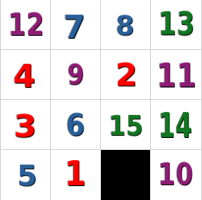
\includegraphics[width=0.25\linewidth]{chapter2/fig/puzzle.png}
	\caption{Example of a sliding puzzle}
	\label{fig:sliding_puzzle}
\end{figure}

\section{Conditions for solvability}
Even and odd sized boards are analysed separately (where size = N).

For odd sized boards where N is odd we have the puzzle only being solvable if and only if the boards
has an even number of inversions. The proof for this can be deduced by looking at Figure 2 and noting that for every switch of the blank block we have an even change in the sum of inversions of the board. \cite{princeton_8puzzle_assignment}

\begin{figure}[!htb]
	\centering
	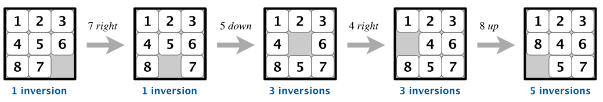
\includegraphics[width=1\linewidth]{chapter2/fig/princeton_odd_boards.png}
	\caption{Odd boards with change in blank piece only having even inversion change \cite{princeton_8puzzle_assignment}}
	\label{fig:sol_odd_board}
\end{figure}

For even sized boards where N is even we have the board solvable if and only if the number of
inversions plus the row of the blank square is odd. This is illustrated in Figure 3.

\begin{figure}[!htb]
	\centering
	\includegraphics[width=1\linewidth]{chapter2/fig/princeton_even_board_solvability.png}
	\caption{Even board solvability \cite{princeton_8puzzle_assignment}}
	\label{fig:sol_even_board}
\end{figure}

Half of all puzzle configurations are unsolvable. \cite{Notes_15_puzzle} This means that we only have N! / 2 configurations
that are solvable for an NxN board. This was proven using parity in the paper in \cite{Notes_15_puzzle}. Sliding puzzles
can be solved relatively quickly with today’s processing of computers for puzzles for example an 5x5
puzzle was solved in 205 tile moves in 2016. \cite{Domain_cube_forum}

The issue more so lies in finding the shortest path to solving a puzzle. This specific problem of solving
with the least amount of tile moves of a sliding puzzle has been defined as NP (non-deterministic polynomial-time) hard. NP hardness is are problems that are as least as hard as NP.
Where in computational complexity theory NP (non-deterministic polynomial-time) is a has a solution
with a proof variable to be in polynomial time by a deterministic Turing Machine. A Turing machine is
a mathematical model defining an abstract machine which manipulates symbols according to a set of
rules. \cite{Computation_finite_and_infinite_machines}

In simpler terms a problem is NP if it can be solved within a time that is a polynomial function of the
input. For instance if we define the time to solve a problem as ‘T’ and the input data as ‘D’. Then as
long as T = polynomial function (D) then a problem is NP.
\graphicspath{{conclusion/fig/}}

\chapter{Summary and Conclusion}
\label{chap:conclusion}

\section{Summary}
Objective 1 ...

Objective 2 ...

Objective 3 ...

So what? Relates back to problem and background sections in introductions.

\section{Future work and reccomendations}

% Bibliography
\bibliography{mybib}

% End matter
\appendix
\chapter{Project Planning Schedule}
\makeatletter\@mkboth{}{Appendix}\makeatother
\label{appen:derivations_bigramseg}

This is an appendix.

\chapter{Outcomes Compliance}
\makeatletter\@mkboth{}{Appendix}\makeatother
\label{appen:derivations_bigramseg}

This is another appendix.

\end{document}

